\documentclass[twoside]{book}

% Packages required by doxygen
\usepackage{calc}
\usepackage{doxygen}
\usepackage{graphicx}
\usepackage[utf8]{inputenc}
\usepackage{makeidx}
\usepackage{multicol}
\usepackage{multirow}
\usepackage{textcomp}
\usepackage[table]{xcolor}

% Font selection
\usepackage[T1]{fontenc}
\usepackage{mathptmx}
\usepackage[scaled=.90]{helvet}
\usepackage{courier}
\usepackage{amssymb}
\usepackage{sectsty}
\renewcommand{\familydefault}{\sfdefault}
\allsectionsfont{%
  \fontseries{bc}\selectfont%
  \color{darkgray}%
}
\renewcommand{\DoxyLabelFont}{%
  \fontseries{bc}\selectfont%
  \color{darkgray}%
}

% Page & text layout
\usepackage{geometry}
\geometry{%
  a4paper,%
  top=2.5cm,%
  bottom=2.5cm,%
  left=2.5cm,%
  right=2.5cm%
}
\tolerance=750
\hfuzz=15pt
\hbadness=750
\setlength{\emergencystretch}{15pt}
\setlength{\parindent}{0cm}
\setlength{\parskip}{0.2cm}
\makeatletter
\renewcommand{\paragraph}{%
  \@startsection{paragraph}{4}{0ex}{-1.0ex}{1.0ex}{%
    \normalfont\normalsize\bfseries\SS@parafont%
  }%
}
\renewcommand{\subparagraph}{%
  \@startsection{subparagraph}{5}{0ex}{-1.0ex}{1.0ex}{%
    \normalfont\normalsize\bfseries\SS@subparafont%
  }%
}
\makeatother

% Headers & footers
\usepackage{fancyhdr}
\pagestyle{fancyplain}
\fancyhead[LE]{\fancyplain{}{\bfseries\thepage}}
\fancyhead[CE]{\fancyplain{}{}}
\fancyhead[RE]{\fancyplain{}{\bfseries\leftmark}}
\fancyhead[LO]{\fancyplain{}{\bfseries\rightmark}}
\fancyhead[CO]{\fancyplain{}{}}
\fancyhead[RO]{\fancyplain{}{\bfseries\thepage}}
\fancyfoot[LE]{\fancyplain{}{}}
\fancyfoot[CE]{\fancyplain{}{}}
\fancyfoot[RE]{\fancyplain{}{\bfseries\scriptsize Generated on Tue Oct 28 2014 13\-:18\-:08 for Shoot The Bully by Doxygen }}
\fancyfoot[LO]{\fancyplain{}{\bfseries\scriptsize Generated on Tue Oct 28 2014 13\-:18\-:08 for Shoot The Bully by Doxygen }}
\fancyfoot[CO]{\fancyplain{}{}}
\fancyfoot[RO]{\fancyplain{}{}}
\renewcommand{\footrulewidth}{0.4pt}
\renewcommand{\chaptermark}[1]{%
  \markboth{#1}{}%
}
\renewcommand{\sectionmark}[1]{%
  \markright{\thesection\ #1}%
}

% Indices & bibliography
\usepackage{natbib}
\usepackage[titles]{tocloft}
\setcounter{tocdepth}{3}
\setcounter{secnumdepth}{5}
\makeindex

% Hyperlinks (required, but should be loaded last)
\usepackage{ifpdf}
\ifpdf
  \usepackage[pdftex,pagebackref=true]{hyperref}
\else
  \usepackage[ps2pdf,pagebackref=true]{hyperref}
\fi
\hypersetup{%
  colorlinks=true,%
  linkcolor=blue,%
  citecolor=blue,%
  unicode%
}

% Custom commands
\newcommand{\clearemptydoublepage}{%
  \newpage{\pagestyle{empty}\cleardoublepage}%
}


%===== C O N T E N T S =====

\begin{document}

% Titlepage & ToC
\hypersetup{pageanchor=false}
\pagenumbering{roman}
\begin{titlepage}
\vspace*{7cm}
\begin{center}%
{\Large Shoot The Bully }\\
\vspace*{1cm}
{\large Generated by Doxygen 1.8.5}\\
\vspace*{0.5cm}
{\small Tue Oct 28 2014 13:18:08}\\
\end{center}
\end{titlepage}
\clearemptydoublepage
\tableofcontents
\clearemptydoublepage
\pagenumbering{arabic}
\hypersetup{pageanchor=true}

%--- Begin generated contents ---
\chapter{Hierarchical Index}
\section{Class Hierarchy}
This inheritance list is sorted roughly, but not completely, alphabetically\-:\begin{DoxyCompactList}
\item exception\begin{DoxyCompactList}
\item \contentsline{section}{end\-Of\-File}{\pageref{classend_of_file}}{}
\item \contentsline{section}{invalid\-Position}{\pageref{classinvalid_position}}{}
\item \contentsline{section}{unknown\-Object}{\pageref{classunknown_object}}{}
\end{DoxyCompactList}
\item \contentsline{section}{Factory}{\pageref{class_factory}}{}
\item \contentsline{section}{Game\-Controller}{\pageref{class_game_controller}}{}
\item \contentsline{section}{Hud\-Controller}{\pageref{class_hud_controller}}{}
\item \contentsline{section}{Level\-Controller\-:\-:Initializer}{\pageref{class_level_controller_1_1_initializer}}{}
\item \contentsline{section}{Input\-Controller}{\pageref{class_input_controller}}{}
\item \contentsline{section}{Level\-Controller}{\pageref{class_level_controller}}{}
\item \contentsline{section}{Sound\-Controller}{\pageref{class_sound_controller}}{}
\item \contentsline{section}{Texture\-Manager}{\pageref{class_texture_manager}}{}
\end{DoxyCompactList}

\chapter{Class Index}
\section{Class List}
Here are the classes, structs, unions and interfaces with brief descriptions\+:\begin{DoxyCompactList}
\item\contentsline{section}{\hyperlink{class_animation}{Animation} }{\pageref{class_animation}}{}
\item\contentsline{section}{\hyperlink{class_bench}{Bench} \\*The \hyperlink{class_bench}{Bench} header file }{\pageref{class_bench}}{}
\item\contentsline{section}{\hyperlink{classbobby_boss}{bobby\+Boss} \\*The Bobby Boss header file }{\pageref{classbobby_boss}}{}
\item\contentsline{section}{\hyperlink{class_bullet}{Bullet} \\*The \hyperlink{class_bullet}{Bullet} header file }{\pageref{class_bullet}}{}
\item\contentsline{section}{\hyperlink{class_checkbox}{Checkbox} \\*The \hyperlink{class_checkbox}{Checkbox} header file }{\pageref{class_checkbox}}{}
\item\contentsline{section}{\hyperlink{class_clickable}{Clickable} \\*The \hyperlink{class_clickable}{Clickable} header file }{\pageref{class_clickable}}{}
\item\contentsline{section}{\hyperlink{class_collision}{Collision} }{\pageref{class_collision}}{}
\item\contentsline{section}{\hyperlink{classdunken_boss}{dunken\+Boss} \\*The Dunken Boss header file }{\pageref{classdunken_boss}}{}
\item\contentsline{section}{\hyperlink{classend_of_file}{end\+Of\+File} \\*The exception header file }{\pageref{classend_of_file}}{}
\item\contentsline{section}{\hyperlink{class_enemy}{Enemy} \\*The \hyperlink{class_enemy}{Enemy} header file }{\pageref{class_enemy}}{}
\item\contentsline{section}{\hyperlink{classethan_boss}{ethan\+Boss} \\*The Ethan Boss header file }{\pageref{classethan_boss}}{}
\item\contentsline{section}{\hyperlink{class_factory}{Factory} }{\pageref{class_factory}}{}
\item\contentsline{section}{\hyperlink{class_game_controller}{Game\+Controller} }{\pageref{class_game_controller}}{}
\item\contentsline{section}{\hyperlink{class_game_object}{Game\+Object} \\*The game object header file }{\pageref{class_game_object}}{}
\item\contentsline{section}{\hyperlink{class_game_object_manager}{Game\+Object\+Manager} \\*The game object manager header file }{\pageref{class_game_object_manager}}{}
\item\contentsline{section}{\hyperlink{class_gun}{Gun} \\*The \hyperlink{class_gun}{Gun} header file }{\pageref{class_gun}}{}
\item\contentsline{section}{\hyperlink{class_hud_controller}{Hud\+Controller} \\*The H\+U\+D\+Controller header file }{\pageref{class_hud_controller}}{}
\item\contentsline{section}{\hyperlink{class_level_controller_1_1_initializer}{Level\+Controller\+::\+Initializer} \\*The initializer is used to initialize some variables in advance }{\pageref{class_level_controller_1_1_initializer}}{}
\item\contentsline{section}{\hyperlink{classinvalid_position}{invalid\+Position} }{\pageref{classinvalid_position}}{}
\item\contentsline{section}{\hyperlink{class_knife}{Knife} \\*The knife header file }{\pageref{class_knife}}{}
\item\contentsline{section}{\hyperlink{class_level_controller}{Level\+Controller} }{\pageref{class_level_controller}}{}
\item\contentsline{section}{\hyperlink{class_logo}{Logo} }{\pageref{class_logo}}{}
\item\contentsline{section}{\hyperlink{class_main_menu}{Main\+Menu} }{\pageref{class_main_menu}}{}
\item\contentsline{section}{\hyperlink{class_music_slider}{Music\+Slider} }{\pageref{class_music_slider}}{}
\item\contentsline{section}{\hyperlink{class_next_round}{Next\+Round} }{\pageref{class_next_round}}{}
\item\contentsline{section}{\hyperlink{class_options}{Options} \\*The header file of the options button }{\pageref{class_options}}{}
\item\contentsline{section}{\hyperlink{classparker_boss}{parker\+Boss} \\*The Parker Boss header file }{\pageref{classparker_boss}}{}
\item\contentsline{section}{\hyperlink{class_particle}{Particle} }{\pageref{class_particle}}{}
\item\contentsline{section}{\hyperlink{class_particle_emitter}{Particle\+Emitter} }{\pageref{class_particle_emitter}}{}
\item\contentsline{section}{\hyperlink{class_particle_manager}{Particle\+Manager} }{\pageref{class_particle_manager}}{}
\item\contentsline{section}{\hyperlink{class_play}{Play} \\*The play header file }{\pageref{class_play}}{}
\item\contentsline{section}{\hyperlink{class_player}{Player} }{\pageref{class_player}}{}
\item\contentsline{section}{\hyperlink{class_powerup}{Powerup} }{\pageref{class_powerup}}{}
\item\contentsline{section}{\hyperlink{structrectangle}{rectangle} }{\pageref{structrectangle}}{}
\item\contentsline{section}{\hyperlink{class_resume}{Resume} \\*The resume header file }{\pageref{class_resume}}{}
\item\contentsline{section}{\hyperlink{class_settings_controller}{Settings\+Controller} \\*The settings controller header file }{\pageref{class_settings_controller}}{}
\item\contentsline{section}{\hyperlink{class_shop}{Shop} \\*The shop header file }{\pageref{class_shop}}{}
\item\contentsline{section}{\hyperlink{class_shop_card}{Shop\+Card} \\*The shop card header file }{\pageref{class_shop_card}}{}
\item\contentsline{section}{\hyperlink{class_slider}{Slider} \\*The slider header file }{\pageref{class_slider}}{}
\item\contentsline{section}{\hyperlink{class_sound_controller}{Sound\+Controller} \\*The sound controller header file }{\pageref{class_sound_controller}}{}
\item\contentsline{section}{\hyperlink{class_sound_slider}{Sound\+Slider} \\*The sound slider header file }{\pageref{class_sound_slider}}{}
\item\contentsline{section}{\hyperlink{classswitch_weapon}{switch\+Weapon} \\*The switch weapon header file }{\pageref{classswitch_weapon}}{}
\item\contentsline{section}{\hyperlink{class_table}{Table} }{\pageref{class_table}}{}
\item\contentsline{section}{\hyperlink{class_texture_manager}{Texture\+Manager} }{\pageref{class_texture_manager}}{}
\item\contentsline{section}{\hyperlink{class_toggle_gore}{Toggle\+Gore} \\*The toggle gore header file }{\pageref{class_toggle_gore}}{}
\item\contentsline{section}{\hyperlink{class_toggle_music}{Toggle\+Music} \\*The toggle music header file }{\pageref{class_toggle_music}}{}
\item\contentsline{section}{\hyperlink{class_toggle_sound}{Toggle\+Sound} \\*The togglesound header file }{\pageref{class_toggle_sound}}{}
\item\contentsline{section}{\hyperlink{class_trashcan}{Trashcan} \\*The \hyperlink{class_trashcan}{Trashcan} header file }{\pageref{class_trashcan}}{}
\item\contentsline{section}{\hyperlink{class_tutorial}{Tutorial} \\*The tutorial header file }{\pageref{class_tutorial}}{}
\item\contentsline{section}{\hyperlink{class_tutorial_screen}{Tutorial\+Screen} \\*The tutorial screen header file }{\pageref{class_tutorial_screen}}{}
\item\contentsline{section}{\hyperlink{class_powerup_1_1_types}{Powerup\+::\+Types} \\*The \hyperlink{class_powerup_1_1_types}{Types} class }{\pageref{class_powerup_1_1_types}}{}
\item\contentsline{section}{\hyperlink{classunknown_object}{unknown\+Object} }{\pageref{classunknown_object}}{}
\item\contentsline{section}{\hyperlink{class_upgrade}{Upgrade} }{\pageref{class_upgrade}}{}
\item\contentsline{section}{\hyperlink{class_weapon}{Weapon} }{\pageref{class_weapon}}{}
\item\contentsline{section}{\hyperlink{class_weapon_card}{Weapon\+Card} \\*The \hyperlink{class_weapon}{Weapon} Card header file }{\pageref{class_weapon_card}}{}
\item\contentsline{section}{\hyperlink{class_weapon_manager}{Weapon\+Manager} }{\pageref{class_weapon_manager}}{}
\item\contentsline{section}{\hyperlink{classzoey_boss}{zoey\+Boss} \\*The Zoey Boss header file }{\pageref{classzoey_boss}}{}
\end{DoxyCompactList}

\chapter{Class Documentation}
\hypertarget{classend_of_file}{\section{end\-Of\-File Class Reference}
\label{classend_of_file}\index{end\-Of\-File@{end\-Of\-File}}
}


The exception header file.  




{\ttfamily \#include $<$Exception.\-h$>$}

Inheritance diagram for end\-Of\-File\-:\begin{figure}[H]
\begin{center}
\leavevmode
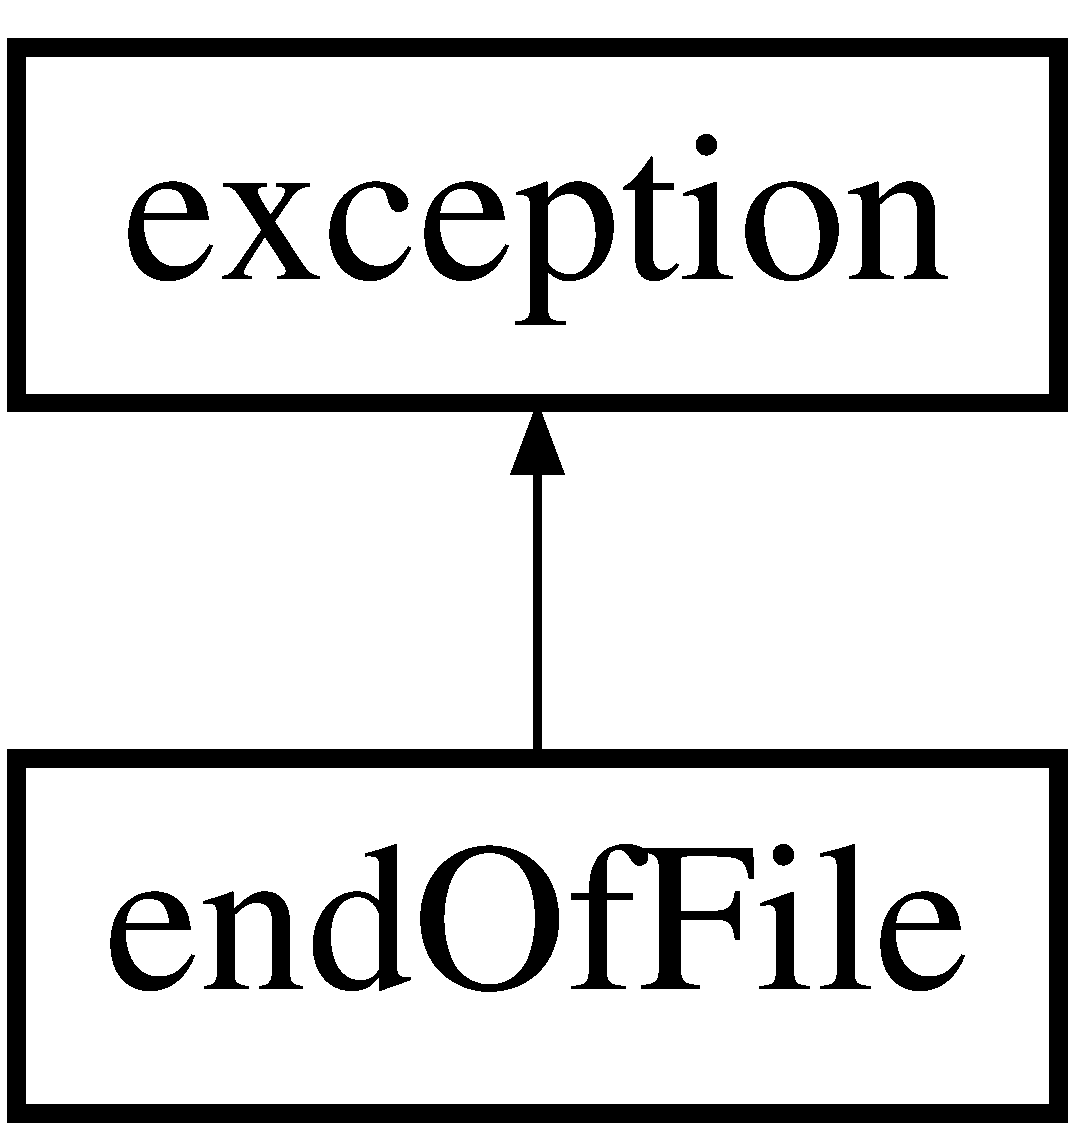
\includegraphics[height=2.000000cm]{classend_of_file}
\end{center}
\end{figure}


\subsection{Detailed Description}
The exception header file. 

This is the header file of the exception class. 

The documentation for this class was generated from the following file\-:\begin{DoxyCompactItemize}
\item 
Exception.\-h\end{DoxyCompactItemize}

\hypertarget{class_factory}{\section{Factory Class Reference}
\label{class_factory}\index{Factory@{Factory}}
}
\subsection*{Public Types}
\begin{DoxyCompactItemize}
\item 
enum \hyperlink{class_factory_a31534970ff95c9cb57a4883cb8ef7b78}{level\-Settings} \{ {\bfseries random} = 256
 \}
\begin{DoxyCompactList}\small\item\em T\-O\-D\-O\-: enum shit idk. \end{DoxyCompactList}\end{DoxyCompactItemize}
\subsection*{Public Member Functions}
\begin{DoxyCompactItemize}
\item 
\hyperlink{class_factory_ac792bf88cfb7b6804b479529da5308cc}{Factory} ()
\begin{DoxyCompactList}\small\item\em The constructor of the factory class. \end{DoxyCompactList}\item 
int \hyperlink{class_factory_af0852710e037ab8ded28cc12ec1c099b}{load\-Level} (std\-::string file)
\begin{DoxyCompactList}\small\item\em The load\-Level method of the factory. \end{DoxyCompactList}\item 
Game\-Object $\ast$ \hyperlink{class_factory_ad7696889634790fcac45cfd18ae44039}{screen\-\_\-object\-\_\-read} (std\-::ifstream \&input, bool to\-Hud)
\begin{DoxyCompactList}\small\item\em The screen\-\_\-object\-\_\-read method of the factory. \end{DoxyCompactList}\item 
\hyperlink{class_factory_a8f71456f48e4df402c778a44191ff40e}{$\sim$\-Factory} ()
\begin{DoxyCompactList}\small\item\em The deconstructor of the factory. \end{DoxyCompactList}\end{DoxyCompactItemize}


\subsection{Constructor \& Destructor Documentation}
\hypertarget{class_factory_ac792bf88cfb7b6804b479529da5308cc}{\index{Factory@{Factory}!Factory@{Factory}}
\index{Factory@{Factory}!Factory@{Factory}}
\subsubsection[{Factory}]{\setlength{\rightskip}{0pt plus 5cm}Factory\-::\-Factory (
\begin{DoxyParamCaption}
{}
\end{DoxyParamCaption}
)}}\label{class_factory_ac792bf88cfb7b6804b479529da5308cc}


The constructor of the factory class. 

default constructor, also initializes the game\-Object\-Manager. \hypertarget{class_factory_a8f71456f48e4df402c778a44191ff40e}{\index{Factory@{Factory}!$\sim$\-Factory@{$\sim$\-Factory}}
\index{$\sim$\-Factory@{$\sim$\-Factory}!Factory@{Factory}}
\subsubsection[{$\sim$\-Factory}]{\setlength{\rightskip}{0pt plus 5cm}Factory\-::$\sim$\-Factory (
\begin{DoxyParamCaption}
{}
\end{DoxyParamCaption}
)}}\label{class_factory_a8f71456f48e4df402c778a44191ff40e}


The deconstructor of the factory. 

the default deconstructor 

\subsection{Member Function Documentation}
\hypertarget{class_factory_af0852710e037ab8ded28cc12ec1c099b}{\index{Factory@{Factory}!load\-Level@{load\-Level}}
\index{load\-Level@{load\-Level}!Factory@{Factory}}
\subsubsection[{load\-Level}]{\setlength{\rightskip}{0pt plus 5cm}int Factory\-::load\-Level (
\begin{DoxyParamCaption}
\item[{std\-::string}]{file}
\end{DoxyParamCaption}
)}}\label{class_factory_af0852710e037ab8ded28cc12ec1c099b}


The load\-Level method of the factory. 

Loads the level from a text file. Puts all items in the map based on the terror level. Also loads all objects to the H\-U\-D. 
\begin{DoxyParams}{Parameters}
{\em file} & The file in which all the game objects are stored. \\
\hline
\end{DoxyParams}
\begin{DoxyReturn}{Returns}
the value of the terror level. 
\end{DoxyReturn}
\hypertarget{class_factory_ad7696889634790fcac45cfd18ae44039}{\index{Factory@{Factory}!screen\-\_\-object\-\_\-read@{screen\-\_\-object\-\_\-read}}
\index{screen\-\_\-object\-\_\-read@{screen\-\_\-object\-\_\-read}!Factory@{Factory}}
\subsubsection[{screen\-\_\-object\-\_\-read}]{\setlength{\rightskip}{0pt plus 5cm}Game\-Object $\ast$ Factory\-::screen\-\_\-object\-\_\-read (
\begin{DoxyParamCaption}
\item[{std\-::ifstream \&}]{input, }
\item[{bool}]{to\-Hud}
\end{DoxyParamCaption}
)}}\label{class_factory_ad7696889634790fcac45cfd18ae44039}


The screen\-\_\-object\-\_\-read method of the factory. 

Reads values from a text file and puts them together to create an object. 
\begin{DoxyParams}{Parameters}
{\em input} & The stream from which the factory has to read the values for the object \\
\hline
{\em to\-Hud} & wether or not the object should be placed on the H\-U\-D \\
\hline
\end{DoxyParams}
\begin{DoxyReturn}{Returns}
the Object created with all the values read from the input stream 
\end{DoxyReturn}


The documentation for this class was generated from the following files\-:\begin{DoxyCompactItemize}
\item 
Factory.\-h\item 
Factory.\-cpp\end{DoxyCompactItemize}

\hypertarget{class_game_controller}{\section{Game\+Controller Class Reference}
\label{class_game_controller}\index{Game\+Controller@{Game\+Controller}}
}
\subsection*{Public Member Functions}
\begin{DoxyCompactItemize}
\item 
float \hyperlink{class_game_controller_a54e8117f438fa872e5c1b24fd9469816}{get\+F\+P\+S} ()
\begin{DoxyCompactList}\small\item\em The get\+F\+P\+S method of the gamecontroller. \end{DoxyCompactList}\item 
void \hyperlink{class_game_controller_af365cd7a71dd76730a0bc92adc092103}{start} ()
\begin{DoxyCompactList}\small\item\em The start method of the gamecontroller. \end{DoxyCompactList}\item 
void \hyperlink{class_game_controller_a97872acdc39172c21e06665854656994}{stop} ()
\begin{DoxyCompactList}\small\item\em The stop method of the gamecontroller. \end{DoxyCompactList}\item 
sf\+::\+Render\+Window \& \hyperlink{class_game_controller_a993ad55478fff868c801ee7e6f4aaa2b}{get\+Window} ()
\begin{DoxyCompactList}\small\item\em The getwindow method of the gamecontroller. \end{DoxyCompactList}\item 
\hypertarget{class_game_controller_a305a4e04f9d2e6232a8a63fe1c6d317e}{sf\+::\+Font $\ast$ {\bfseries get\+Font} ()}\label{class_game_controller_a305a4e04f9d2e6232a8a63fe1c6d317e}

\item 
\hypertarget{class_game_controller_aab436961a422d078975bc7a49bdfcab7}{\hyperlink{class_game_controller_aab436961a422d078975bc7a49bdfcab7}{$\sim$\+Game\+Controller} ()}\label{class_game_controller_aab436961a422d078975bc7a49bdfcab7}

\begin{DoxyCompactList}\small\item\em The deconstructor of the gamecontroller. \end{DoxyCompactList}\end{DoxyCompactItemize}
\subsection*{Static Public Member Functions}
\begin{DoxyCompactItemize}
\item 
static \hyperlink{class_game_controller}{Game\+Controller} \& \hyperlink{class_game_controller_a38f17e349f91955d10c9d8511b245e9c}{get\+Instance} ()
\begin{DoxyCompactList}\small\item\em The get\+Instance method of the gamecontroller. \end{DoxyCompactList}\end{DoxyCompactItemize}


\subsection{Member Function Documentation}
\hypertarget{class_game_controller_a54e8117f438fa872e5c1b24fd9469816}{\index{Game\+Controller@{Game\+Controller}!get\+F\+P\+S@{get\+F\+P\+S}}
\index{get\+F\+P\+S@{get\+F\+P\+S}!Game\+Controller@{Game\+Controller}}
\subsubsection[{get\+F\+P\+S}]{\setlength{\rightskip}{0pt plus 5cm}float Game\+Controller\+::get\+F\+P\+S (
\begin{DoxyParamCaption}
{}
\end{DoxyParamCaption}
)}}\label{class_game_controller_a54e8117f438fa872e5c1b24fd9469816}


The get\+F\+P\+S method of the gamecontroller. 

\begin{DoxyReturn}{Returns}
The frames per second of the game 
\end{DoxyReturn}
\hypertarget{class_game_controller_a38f17e349f91955d10c9d8511b245e9c}{\index{Game\+Controller@{Game\+Controller}!get\+Instance@{get\+Instance}}
\index{get\+Instance@{get\+Instance}!Game\+Controller@{Game\+Controller}}
\subsubsection[{get\+Instance}]{\setlength{\rightskip}{0pt plus 5cm}static {\bf Game\+Controller}\& Game\+Controller\+::get\+Instance (
\begin{DoxyParamCaption}
{}
\end{DoxyParamCaption}
)\hspace{0.3cm}{\ttfamily [inline]}, {\ttfamily [static]}}}\label{class_game_controller_a38f17e349f91955d10c9d8511b245e9c}


The get\+Instance method of the gamecontroller. 

This method makes sure there is only 1 instance of the gamecontroller at a time. This way, every time an external class uses a gamecontroller, it uses a gamecontroller with the same attributes as every other class. \begin{DoxyReturn}{Returns}
The instance of the gamecontroller 
\end{DoxyReturn}
\hypertarget{class_game_controller_a993ad55478fff868c801ee7e6f4aaa2b}{\index{Game\+Controller@{Game\+Controller}!get\+Window@{get\+Window}}
\index{get\+Window@{get\+Window}!Game\+Controller@{Game\+Controller}}
\subsubsection[{get\+Window}]{\setlength{\rightskip}{0pt plus 5cm}sf\+::\+Render\+Window \& Game\+Controller\+::get\+Window (
\begin{DoxyParamCaption}
{}
\end{DoxyParamCaption}
)}}\label{class_game_controller_a993ad55478fff868c801ee7e6f4aaa2b}


The getwindow method of the gamecontroller. 

\begin{DoxyReturn}{Returns}
The current window the game has to be drawn in 
\end{DoxyReturn}
\hypertarget{class_game_controller_af365cd7a71dd76730a0bc92adc092103}{\index{Game\+Controller@{Game\+Controller}!start@{start}}
\index{start@{start}!Game\+Controller@{Game\+Controller}}
\subsubsection[{start}]{\setlength{\rightskip}{0pt plus 5cm}void Game\+Controller\+::start (
\begin{DoxyParamCaption}
{}
\end{DoxyParamCaption}
)}}\label{class_game_controller_af365cd7a71dd76730a0bc92adc092103}


The start method of the gamecontroller. 

Calling this method will cause the game to start running. \hypertarget{class_game_controller_a97872acdc39172c21e06665854656994}{\index{Game\+Controller@{Game\+Controller}!stop@{stop}}
\index{stop@{stop}!Game\+Controller@{Game\+Controller}}
\subsubsection[{stop}]{\setlength{\rightskip}{0pt plus 5cm}void Game\+Controller\+::stop (
\begin{DoxyParamCaption}
{}
\end{DoxyParamCaption}
)}}\label{class_game_controller_a97872acdc39172c21e06665854656994}


The stop method of the gamecontroller. 

Calling this method will stop the game. Prerequirement\+: the game has to be started. 

The documentation for this class was generated from the following files\+:\begin{DoxyCompactItemize}
\item 
Game\+Controller.\+h\item 
Game\+Controller.\+cpp\end{DoxyCompactItemize}

\hypertarget{class_hud_controller}{\section{Hud\-Controller Class Reference}
\label{class_hud_controller}\index{Hud\-Controller@{Hud\-Controller}}
}


The H\-U\-D\-Controller header file.  




{\ttfamily \#include $<$Hud\-Controller.\-h$>$}

\subsection*{Public Member Functions}
\begin{DoxyCompactItemize}
\item 
void \hyperlink{class_hud_controller_a27862a3db822f65de6dbcf22835ec58a}{add\-Object} (Game\-Object $\ast$object)
\begin{DoxyCompactList}\small\item\em The add object method of the H\-U\-D controller. \end{DoxyCompactList}\item 
void \hyperlink{class_hud_controller_abaab3a30a47733b2588236100267e206}{add\-Object\-From\-Factory} (Game\-Object $\ast$object)
\begin{DoxyCompactList}\small\item\em The add object from factory method of the hud controller. \end{DoxyCompactList}\item 
void \hyperlink{class_hud_controller_ab07bc4161257a8fbc16df56ed9dbf1ea}{remove\-Object} (Game\-Object $\ast$object)
\begin{DoxyCompactList}\small\item\em The remove object method of the hud controller. \end{DoxyCompactList}\item 
void \hyperlink{class_hud_controller_aac63180083695594ae2d17278c13d604}{remove\-All\-Objects} (Game\-Object $\ast$object)
\begin{DoxyCompactList}\small\item\em The remove all objects method of the hud controller. \end{DoxyCompactList}\item 
void \hyperlink{class_hud_controller_abeeed176eb5114ce613c499135c528d4}{load} ()
\begin{DoxyCompactList}\small\item\em The load method of the hud controller. \end{DoxyCompactList}\item 
void \hyperlink{class_hud_controller_a6cd82988ca9221b6cb8d520a8e26b204}{step} (sf\-::\-Render\-Window \&window)
\begin{DoxyCompactList}\small\item\em The step method of the H\-U\-D controller. \end{DoxyCompactList}\item 
sf\-::\-Vector2f \hyperlink{class_hud_controller_a4c6c9c53841c41d156a2f715a43be703}{get\-Mouse\-Pos} ()
\begin{DoxyCompactList}\small\item\em the get mouse position method of the hud controller \end{DoxyCompactList}\item 
void \hyperlink{class_hud_controller_a9e9c4e19bdb0bc55247c96e79c5548c3}{prepare\-For\-Next\-Level} ()
\begin{DoxyCompactList}\small\item\em the prepare for next level method of the hud controller \end{DoxyCompactList}\item 
\hyperlink{class_hud_controller_a53264716b1a602a351a7bfcebb0d4dc1}{$\sim$\-Hud\-Controller} ()
\begin{DoxyCompactList}\small\item\em the deconstructor of the hud controller \end{DoxyCompactList}\end{DoxyCompactItemize}
\subsection*{Static Public Member Functions}
\begin{DoxyCompactItemize}
\item 
static \hyperlink{class_hud_controller}{Hud\-Controller} \& \hyperlink{class_hud_controller_a9dafa97894bb74e7ada5ab5f76b886c4}{get\-Instance} ()
\begin{DoxyCompactList}\small\item\em The get\-Insatnce method of the H\-U\-D controller. \end{DoxyCompactList}\end{DoxyCompactItemize}


\subsection{Detailed Description}
The H\-U\-D\-Controller header file. 

This is the header file of the H\-U\-D controller class. 

\subsection{Constructor \& Destructor Documentation}
\hypertarget{class_hud_controller_a53264716b1a602a351a7bfcebb0d4dc1}{\index{Hud\-Controller@{Hud\-Controller}!$\sim$\-Hud\-Controller@{$\sim$\-Hud\-Controller}}
\index{$\sim$\-Hud\-Controller@{$\sim$\-Hud\-Controller}!HudController@{Hud\-Controller}}
\subsubsection[{$\sim$\-Hud\-Controller}]{\setlength{\rightskip}{0pt plus 5cm}Hud\-Controller\-::$\sim$\-Hud\-Controller (
\begin{DoxyParamCaption}
{}
\end{DoxyParamCaption}
)\hspace{0.3cm}{\ttfamily [inline]}}}\label{class_hud_controller_a53264716b1a602a351a7bfcebb0d4dc1}


the deconstructor of the hud controller 

default 

\subsection{Member Function Documentation}
\hypertarget{class_hud_controller_a27862a3db822f65de6dbcf22835ec58a}{\index{Hud\-Controller@{Hud\-Controller}!add\-Object@{add\-Object}}
\index{add\-Object@{add\-Object}!HudController@{Hud\-Controller}}
\subsubsection[{add\-Object}]{\setlength{\rightskip}{0pt plus 5cm}void Hud\-Controller\-::add\-Object (
\begin{DoxyParamCaption}
\item[{Game\-Object $\ast$}]{object}
\end{DoxyParamCaption}
)}}\label{class_hud_controller_a27862a3db822f65de6dbcf22835ec58a}


The add object method of the H\-U\-D controller. 

This function will put a new game object under the control of the game controller 
\begin{DoxyParams}{Parameters}
{\em object} & The object that has to be added \\
\hline
\end{DoxyParams}
\hypertarget{class_hud_controller_abaab3a30a47733b2588236100267e206}{\index{Hud\-Controller@{Hud\-Controller}!add\-Object\-From\-Factory@{add\-Object\-From\-Factory}}
\index{add\-Object\-From\-Factory@{add\-Object\-From\-Factory}!HudController@{Hud\-Controller}}
\subsubsection[{add\-Object\-From\-Factory}]{\setlength{\rightskip}{0pt plus 5cm}void Hud\-Controller\-::add\-Object\-From\-Factory (
\begin{DoxyParamCaption}
\item[{Game\-Object $\ast$}]{object}
\end{DoxyParamCaption}
)}}\label{class_hud_controller_abaab3a30a47733b2588236100267e206}


The add object from factory method of the hud controller. 

Puts an object created by the factory under control of the game controller 
\begin{DoxyParams}{Parameters}
{\em object} & The object from the factory \\
\hline
\end{DoxyParams}
\hypertarget{class_hud_controller_a9dafa97894bb74e7ada5ab5f76b886c4}{\index{Hud\-Controller@{Hud\-Controller}!get\-Instance@{get\-Instance}}
\index{get\-Instance@{get\-Instance}!HudController@{Hud\-Controller}}
\subsubsection[{get\-Instance}]{\setlength{\rightskip}{0pt plus 5cm}static {\bf Hud\-Controller}\& Hud\-Controller\-::get\-Instance (
\begin{DoxyParamCaption}
{}
\end{DoxyParamCaption}
)\hspace{0.3cm}{\ttfamily [inline]}, {\ttfamily [static]}}}\label{class_hud_controller_a9dafa97894bb74e7ada5ab5f76b886c4}


The get\-Insatnce method of the H\-U\-D controller. 

This method makes sure there is only 1 instance of the H\-U\-D controller at a time. This way, every time an external class uses a H\-U\-D controller, it uses a H\-U\-D controller with the same attributes as every other class. \begin{DoxyReturn}{Returns}
The instance of the H\-U\-D controller 
\end{DoxyReturn}
\hypertarget{class_hud_controller_a4c6c9c53841c41d156a2f715a43be703}{\index{Hud\-Controller@{Hud\-Controller}!get\-Mouse\-Pos@{get\-Mouse\-Pos}}
\index{get\-Mouse\-Pos@{get\-Mouse\-Pos}!HudController@{Hud\-Controller}}
\subsubsection[{get\-Mouse\-Pos}]{\setlength{\rightskip}{0pt plus 5cm}sf\-::\-Vector2f Hud\-Controller\-::get\-Mouse\-Pos (
\begin{DoxyParamCaption}
{}
\end{DoxyParamCaption}
)}}\label{class_hud_controller_a4c6c9c53841c41d156a2f715a43be703}


the get mouse position method of the hud controller 

\begin{DoxyReturn}{Returns}
The position of the mouse cursor. 
\end{DoxyReturn}
\hypertarget{class_hud_controller_abeeed176eb5114ce613c499135c528d4}{\index{Hud\-Controller@{Hud\-Controller}!load@{load}}
\index{load@{load}!HudController@{Hud\-Controller}}
\subsubsection[{load}]{\setlength{\rightskip}{0pt plus 5cm}void Hud\-Controller\-::load (
\begin{DoxyParamCaption}
{}
\end{DoxyParamCaption}
)}}\label{class_hud_controller_abeeed176eb5114ce613c499135c528d4}


The load method of the hud controller. 

This method will set all the standard values for the H\-U\-D objects. \hypertarget{class_hud_controller_a9e9c4e19bdb0bc55247c96e79c5548c3}{\index{Hud\-Controller@{Hud\-Controller}!prepare\-For\-Next\-Level@{prepare\-For\-Next\-Level}}
\index{prepare\-For\-Next\-Level@{prepare\-For\-Next\-Level}!HudController@{Hud\-Controller}}
\subsubsection[{prepare\-For\-Next\-Level}]{\setlength{\rightskip}{0pt plus 5cm}void Hud\-Controller\-::prepare\-For\-Next\-Level (
\begin{DoxyParamCaption}
{}
\end{DoxyParamCaption}
)}}\label{class_hud_controller_a9e9c4e19bdb0bc55247c96e79c5548c3}


the prepare for next level method of the hud controller 

deletes all the objects from the H\-U\-D to make place for the new objects of the next level \hypertarget{class_hud_controller_aac63180083695594ae2d17278c13d604}{\index{Hud\-Controller@{Hud\-Controller}!remove\-All\-Objects@{remove\-All\-Objects}}
\index{remove\-All\-Objects@{remove\-All\-Objects}!HudController@{Hud\-Controller}}
\subsubsection[{remove\-All\-Objects}]{\setlength{\rightskip}{0pt plus 5cm}void Hud\-Controller\-::remove\-All\-Objects (
\begin{DoxyParamCaption}
\item[{Game\-Object $\ast$}]{object}
\end{DoxyParamCaption}
)}}\label{class_hud_controller_aac63180083695594ae2d17278c13d604}


The remove all objects method of the hud controller. 

This method will remove the complete list of game objects 
\begin{DoxyParams}{Parameters}
{\em object} & The pointer to the start of the object vector \\
\hline
\end{DoxyParams}
\hypertarget{class_hud_controller_ab07bc4161257a8fbc16df56ed9dbf1ea}{\index{Hud\-Controller@{Hud\-Controller}!remove\-Object@{remove\-Object}}
\index{remove\-Object@{remove\-Object}!HudController@{Hud\-Controller}}
\subsubsection[{remove\-Object}]{\setlength{\rightskip}{0pt plus 5cm}void Hud\-Controller\-::remove\-Object (
\begin{DoxyParamCaption}
\item[{Game\-Object $\ast$}]{object}
\end{DoxyParamCaption}
)}}\label{class_hud_controller_ab07bc4161257a8fbc16df56ed9dbf1ea}


The remove object method of the hud controller. 

This function will remove a game object under the control of the game controller, and will destroy this particular game object. 
\begin{DoxyParams}{Parameters}
{\em object} & The object that has to be removed \\
\hline
\end{DoxyParams}
\hypertarget{class_hud_controller_a6cd82988ca9221b6cb8d520a8e26b204}{\index{Hud\-Controller@{Hud\-Controller}!step@{step}}
\index{step@{step}!HudController@{Hud\-Controller}}
\subsubsection[{step}]{\setlength{\rightskip}{0pt plus 5cm}void Hud\-Controller\-::step (
\begin{DoxyParamCaption}
\item[{sf\-::\-Render\-Window \&}]{window}
\end{DoxyParamCaption}
)}}\label{class_hud_controller_a6cd82988ca9221b6cb8d520a8e26b204}


The step method of the H\-U\-D controller. 

This method will update every object from the H\-U\-D and draw them 
\begin{DoxyParams}{Parameters}
{\em window} & The window on which the objects have to be drawn \\
\hline
\end{DoxyParams}


The documentation for this class was generated from the following files\-:\begin{DoxyCompactItemize}
\item 
Hud\-Controller.\-h\item 
Hud\-Controller.\-cpp\end{DoxyCompactItemize}

\hypertarget{class_level_controller_1_1_initializer}{\section{Level\+Controller\+:\+:Initializer Class Reference}
\label{class_level_controller_1_1_initializer}\index{Level\+Controller\+::\+Initializer@{Level\+Controller\+::\+Initializer}}
}
\subsection*{Public Member Functions}
\begin{DoxyCompactItemize}
\item 
\hypertarget{class_level_controller_1_1_initializer_a12f38f31c04a35ea21f977883eb6f4d5}{{\bfseries Initializer} (std\+::string name)}\label{class_level_controller_1_1_initializer_a12f38f31c04a35ea21f977883eb6f4d5}

\end{DoxyCompactItemize}
\subsection*{Public Attributes}
\begin{DoxyCompactItemize}
\item 
\hypertarget{class_level_controller_1_1_initializer_ac90a27c67674791807041b13124426c7}{std\+::string {\bfseries name}}\label{class_level_controller_1_1_initializer_ac90a27c67674791807041b13124426c7}

\end{DoxyCompactItemize}


The documentation for this class was generated from the following files\+:\begin{DoxyCompactItemize}
\item 
Level\+Controller.\+h\item 
Level\+Controller.\+cpp\end{DoxyCompactItemize}

\hypertarget{class_input_controller}{\section{Input\+Controller Class Reference}
\label{class_input_controller}\index{Input\+Controller@{Input\+Controller}}
}


The documentation for this class was generated from the following file\+:\begin{DoxyCompactItemize}
\item 
Input\+Controller.\+h\end{DoxyCompactItemize}

\hypertarget{classinvalid_position}{\section{invalid\-Position Class Reference}
\label{classinvalid_position}\index{invalid\-Position@{invalid\-Position}}
}
Inheritance diagram for invalid\-Position\-:\begin{figure}[H]
\begin{center}
\leavevmode
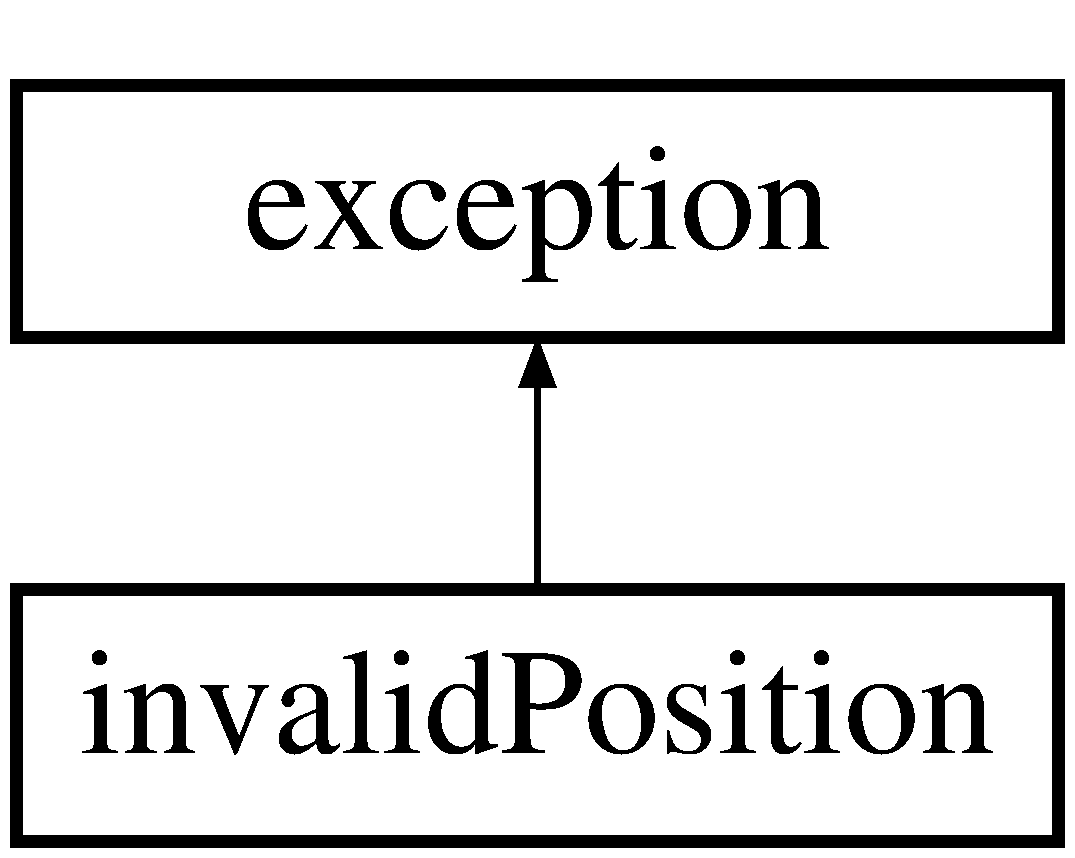
\includegraphics[height=2.000000cm]{classinvalid_position}
\end{center}
\end{figure}
\subsection*{Public Member Functions}
\begin{DoxyCompactItemize}
\item 
\hyperlink{classinvalid_position_a8c8ae14d696ff3de5e292c65a2d00c25}{invalid\-Position} (char c)
\begin{DoxyCompactList}\small\item\em The constructor of the \hyperlink{classinvalid_position}{invalid\-Position} exception. \end{DoxyCompactList}\item 
\hypertarget{classinvalid_position_a07a9ba0700b246c757a9e22ca9572b4b}{const char $\ast$ \hyperlink{classinvalid_position_a07a9ba0700b246c757a9e22ca9572b4b}{what} () const override}\label{classinvalid_position_a07a9ba0700b246c757a9e22ca9572b4b}

\begin{DoxyCompactList}\small\item\em The \hyperlink{classinvalid_position_a07a9ba0700b246c757a9e22ca9572b4b}{what()} method of an exception returns a string stating the exception. \end{DoxyCompactList}\end{DoxyCompactItemize}


\subsection{Constructor \& Destructor Documentation}
\hypertarget{classinvalid_position_a8c8ae14d696ff3de5e292c65a2d00c25}{\index{invalid\-Position@{invalid\-Position}!invalid\-Position@{invalid\-Position}}
\index{invalid\-Position@{invalid\-Position}!invalidPosition@{invalid\-Position}}
\subsubsection[{invalid\-Position}]{\setlength{\rightskip}{0pt plus 5cm}invalid\-Position\-::invalid\-Position (
\begin{DoxyParamCaption}
\item[{char}]{c}
\end{DoxyParamCaption}
)}}\label{classinvalid_position_a8c8ae14d696ff3de5e292c65a2d00c25}


The constructor of the \hyperlink{classinvalid_position}{invalid\-Position} exception. 

Creates a string which tells what character has an invalid position. 

The documentation for this class was generated from the following files\-:\begin{DoxyCompactItemize}
\item 
Exception.\-h\item 
Exception.\-cpp\end{DoxyCompactItemize}

\hypertarget{class_level_controller}{\section{Level\+Controller Class Reference}
\label{class_level_controller}\index{Level\+Controller@{Level\+Controller}}
}


Collaboration diagram for Level\+Controller\+:
\nopagebreak
\begin{figure}[H]
\begin{center}
\leavevmode
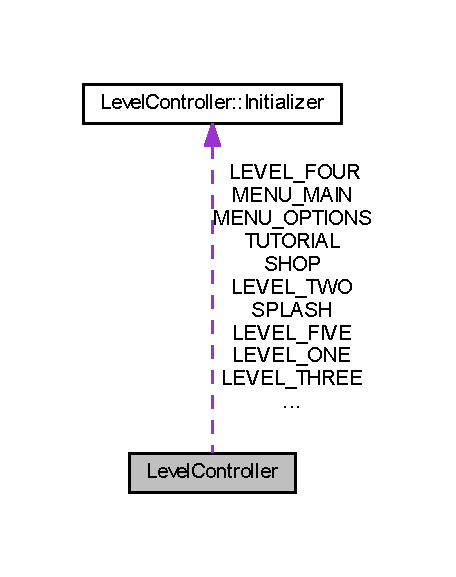
\includegraphics[width=219pt]{class_level_controller__coll__graph}
\end{center}
\end{figure}
\subsection*{Classes}
\begin{DoxyCompactItemize}
\item 
class \hyperlink{class_level_controller_1_1_initializer}{Initializer}
\begin{DoxyCompactList}\small\item\em The initializer is used to initialize some variables in advance. \end{DoxyCompactList}\end{DoxyCompactItemize}
\subsection*{Public Member Functions}
\begin{DoxyCompactItemize}
\item 
void \hyperlink{class_level_controller_a9cb1f95fee01739d9658801dfebb43b1}{go\+To\+Next\+Level} (\hyperlink{class_level_controller_1_1_initializer}{Level\+Controller\+::\+Initializer} $\ast$initializer)
\begin{DoxyCompactList}\small\item\em The go to next level method of the level controller. \end{DoxyCompactList}\item 
void \hyperlink{class_level_controller_a0b8f10e66f7b97615c92340e10f77a07}{start\+Level} (\hyperlink{class_level_controller_1_1_initializer}{Level\+Controller\+::\+Initializer} initializer)
\begin{DoxyCompactList}\small\item\em The start level method of the level controller. \end{DoxyCompactList}\item 
void \hyperlink{class_level_controller_a1235128f78023483b022bab8e2b0125c}{set\+Zoom} (float f)
\begin{DoxyCompactList}\small\item\em The set zoom method of the level controller. \end{DoxyCompactList}\item 
void \hyperlink{class_level_controller_a230987fb618cc9949974a4f4b994bbc1}{add\+Object} (\hyperlink{class_game_object}{Game\+Object} $\ast$object)
\begin{DoxyCompactList}\small\item\em The add Object method of the level controller. \end{DoxyCompactList}\item 
void \hyperlink{class_level_controller_afd60c294955bc06dafac9f5ea146c53d}{add\+Object\+From\+Factory} (\hyperlink{class_game_object}{Game\+Object} $\ast$object)
\begin{DoxyCompactList}\small\item\em The add object from factory method of the level controller. \end{DoxyCompactList}\item 
void \hyperlink{class_level_controller_ad8894683730d484c0ba359c0ee88b219}{remove\+Object} (\hyperlink{class_game_object}{Game\+Object} $\ast$object)
\begin{DoxyCompactList}\small\item\em The remove object method of the level controller. \end{DoxyCompactList}\item 
void \hyperlink{class_level_controller_a3f33f48f2476ad4a68ad5880ea02db22}{remove\+All\+Objects} (\hyperlink{class_game_object}{Game\+Object} $\ast$object)
\begin{DoxyCompactList}\small\item\em The remove all objects method of the level controller. \end{DoxyCompactList}\item 
void \hyperlink{class_level_controller_abd5d6b2ae138b8e086e890fddf46ccef}{move\+Main\+View} (sf\+::\+Vector2f pos)
\begin{DoxyCompactList}\small\item\em The move main view method of the level controller. \end{DoxyCompactList}\item 
void \hyperlink{class_level_controller_a02c383a82a966cb4c0a53d571e771016}{move\+Main\+View} (float x, float y)
\begin{DoxyCompactList}\small\item\em the move main view method using two coordinates \end{DoxyCompactList}\item 
void \hyperlink{class_level_controller_a18cdb3e6d6f3d6e9dde4de2c21bc99cf}{set\+Main\+View} (sf\+::\+Vector2f pos)
\begin{DoxyCompactList}\small\item\em The set\+Main view method of the level controller. \end{DoxyCompactList}\item 
void \hyperlink{class_level_controller_a60cba41df915fcfa0fbb4bff105923e0}{set\+Main\+View} (float x, float y)
\begin{DoxyCompactList}\small\item\em The set main view method. \end{DoxyCompactList}\item 
void \hyperlink{class_level_controller_a57e12d591397a1ab9c2641abf2b5fa9d}{set\+Paused} ()
\begin{DoxyCompactList}\small\item\em The set paused method of the level controller. \end{DoxyCompactList}\item 
void \hyperlink{class_level_controller_acc3a82f2de457b3cb3863c5bb49a909c}{step} (float fps, sf\+::\+Render\+Window \&window)
\begin{DoxyCompactList}\small\item\em The step method of the level controller. \end{DoxyCompactList}\item 
void \hyperlink{class_level_controller_a5d7b9ef50353a7d1e357632180ce75e5}{reset} ()
\begin{DoxyCompactList}\small\item\em The reset method of the level controller. \end{DoxyCompactList}\item 
\hyperlink{class_player}{Player} $\ast$ \hyperlink{class_level_controller_a203ded80ef03720a9e9069d54e500689}{get\+Player} ()
\begin{DoxyCompactList}\small\item\em The get player method of the level controller. \end{DoxyCompactList}\item 
\hyperlink{class_player}{Player} $\ast$ \hyperlink{class_level_controller_a327a14ec720c334f0f6c92ae3ad33924}{get\+Player2} ()
\begin{DoxyCompactList}\small\item\em The second get player method. \end{DoxyCompactList}\item 
\hyperlink{class_particle_manager}{Particle\+Manager} $\ast$ \hyperlink{class_level_controller_a8e3f9f2081f00f3e1ade44eb7e8c24ad}{get\+Particle\+Manager} ()
\begin{DoxyCompactList}\small\item\em The get particle manager method of the level controller. \end{DoxyCompactList}\item 
sf\+::\+Vector2f \hyperlink{class_level_controller_ac08e5cb1592d8e7378253732e9989801}{get\+Mouse\+Pos} ()
\begin{DoxyCompactList}\small\item\em The get mouse position method of the level controller. \end{DoxyCompactList}\item 
const std\+::vector$<$ \hyperlink{class_game_object}{Game\+Object} $\ast$ $>$ \hyperlink{class_level_controller_a331dc36b48234e99d07a6db68e700297}{get\+Game\+Objects} ()
\begin{DoxyCompactList}\small\item\em The get game objects method of the level controller. \end{DoxyCompactList}\item 
void \hyperlink{class_level_controller_a77c7be37cbb30dc3ff6574c053562260}{go\+To\+Next\+Round} ()
\begin{DoxyCompactList}\small\item\em The go to next round method. \end{DoxyCompactList}\end{DoxyCompactItemize}
\subsection*{Static Public Member Functions}
\begin{DoxyCompactItemize}
\item 
static \hyperlink{class_level_controller}{Level\+Controller} \& \hyperlink{class_level_controller_aff1d9aba9f9fb043e644cc4c01869b7f}{get\+Instance} ()
\begin{DoxyCompactList}\small\item\em The get instance method of the level controller. \end{DoxyCompactList}\end{DoxyCompactItemize}
\subsection*{Public Attributes}
\begin{DoxyCompactItemize}
\item 
\hypertarget{class_level_controller_aed3a20ba260b3562516561bc065fd3de}{\hyperlink{class_level_controller_1_1_initializer}{Level\+Controller\+::\+Initializer} \hyperlink{class_level_controller_aed3a20ba260b3562516561bc065fd3de}{L\+E\+V\+E\+L\+\_\+\+O\+N\+E} \{ \char`\"{}Resources/Levels/level\+One.\+level\char`\"{} \}}\label{class_level_controller_aed3a20ba260b3562516561bc065fd3de}

\begin{DoxyCompactList}\small\item\em The location of the level one file. \end{DoxyCompactList}\item 
\hypertarget{class_level_controller_a83feeec328501b067d422301c5b5cea6}{\hyperlink{class_level_controller_1_1_initializer}{Level\+Controller\+::\+Initializer} \hyperlink{class_level_controller_a83feeec328501b067d422301c5b5cea6}{L\+E\+V\+E\+L\+\_\+\+T\+W\+O} \{ \char`\"{}Resources/Levels/level\+Two.\+level\char`\"{} \}}\label{class_level_controller_a83feeec328501b067d422301c5b5cea6}

\begin{DoxyCompactList}\small\item\em The location of the level two file. \end{DoxyCompactList}\item 
\hypertarget{class_level_controller_a0d73c813ab9ed413b8821c19d03e4b2e}{\hyperlink{class_level_controller_1_1_initializer}{Level\+Controller\+::\+Initializer} \hyperlink{class_level_controller_a0d73c813ab9ed413b8821c19d03e4b2e}{L\+E\+V\+E\+L\+\_\+\+T\+H\+R\+E\+E} \{ \char`\"{}Resources/Levels/level\+Three.\+level\char`\"{} \}}\label{class_level_controller_a0d73c813ab9ed413b8821c19d03e4b2e}

\begin{DoxyCompactList}\small\item\em The location of the level three file. \end{DoxyCompactList}\item 
\hypertarget{class_level_controller_af795ecf4216b61bcb8068ec80d2a2246}{\hyperlink{class_level_controller_1_1_initializer}{Level\+Controller\+::\+Initializer} \hyperlink{class_level_controller_af795ecf4216b61bcb8068ec80d2a2246}{L\+E\+V\+E\+L\+\_\+\+F\+O\+U\+R} \{ \char`\"{}Resources/Levels/level\+Four.\+level\char`\"{} \}}\label{class_level_controller_af795ecf4216b61bcb8068ec80d2a2246}

\begin{DoxyCompactList}\small\item\em The location of the level four file. \end{DoxyCompactList}\item 
\hypertarget{class_level_controller_a634c5a8bde652242d217999ddc743e6d}{\hyperlink{class_level_controller_1_1_initializer}{Level\+Controller\+::\+Initializer} \hyperlink{class_level_controller_a634c5a8bde652242d217999ddc743e6d}{L\+E\+V\+E\+L\+\_\+\+F\+I\+V\+E} \{ \char`\"{}Resources/Levels/level\+Five.\+level\char`\"{} \}}\label{class_level_controller_a634c5a8bde652242d217999ddc743e6d}

\begin{DoxyCompactList}\small\item\em The location of the level five file. \end{DoxyCompactList}\item 
\hypertarget{class_level_controller_ad4835322127c6b5d093be8f8ea1735bd}{\hyperlink{class_level_controller_1_1_initializer}{Level\+Controller\+::\+Initializer} \hyperlink{class_level_controller_ad4835322127c6b5d093be8f8ea1735bd}{M\+E\+N\+U\+\_\+\+M\+A\+I\+N} \{ \char`\"{}Resources/Levels/main\+Menu.\+level\char`\"{} \}}\label{class_level_controller_ad4835322127c6b5d093be8f8ea1735bd}

\begin{DoxyCompactList}\small\item\em The location of the file containing the main menu. \end{DoxyCompactList}\item 
\hypertarget{class_level_controller_a062b3091693fbfeb9140431659899ad7}{\hyperlink{class_level_controller_1_1_initializer}{Level\+Controller\+::\+Initializer} \hyperlink{class_level_controller_a062b3091693fbfeb9140431659899ad7}{M\+E\+N\+U\+\_\+\+O\+P\+T\+I\+O\+N\+S} \{ \char`\"{}Resources/Levels/options\+Menu.\+level\char`\"{} \}}\label{class_level_controller_a062b3091693fbfeb9140431659899ad7}

\begin{DoxyCompactList}\small\item\em The location of the file containing the options menu. \end{DoxyCompactList}\item 
\hypertarget{class_level_controller_a3cc829ed89f8a4fad54369bcdb10e985}{\hyperlink{class_level_controller_1_1_initializer}{Level\+Controller\+::\+Initializer} \hyperlink{class_level_controller_a3cc829ed89f8a4fad54369bcdb10e985}{S\+H\+O\+P} \{ \char`\"{}Resources/Levels/shop.\+level\char`\"{} \}}\label{class_level_controller_a3cc829ed89f8a4fad54369bcdb10e985}

\begin{DoxyCompactList}\small\item\em The location of the file containing the shop level. \end{DoxyCompactList}\item 
\hypertarget{class_level_controller_ab0acb0362eba763e16c89d694f97d7f7}{\hyperlink{class_level_controller_1_1_initializer}{Level\+Controller\+::\+Initializer} \hyperlink{class_level_controller_ab0acb0362eba763e16c89d694f97d7f7}{T\+U\+T\+O\+R\+I\+A\+L} \{ \char`\"{}Resources/Levels/tutorial.\+level\char`\"{} \}}\label{class_level_controller_ab0acb0362eba763e16c89d694f97d7f7}

\begin{DoxyCompactList}\small\item\em The location of the file containing the tutorial level. \end{DoxyCompactList}\item 
\hypertarget{class_level_controller_a74aa85b7436b80624576389e3b826aca}{\hyperlink{class_level_controller_1_1_initializer}{Level\+Controller\+::\+Initializer} \hyperlink{class_level_controller_a74aa85b7436b80624576389e3b826aca}{S\+P\+L\+A\+S\+H} \{ \char`\"{}Resources/Levels/logo.\+level\char`\"{} \}}\label{class_level_controller_a74aa85b7436b80624576389e3b826aca}

\begin{DoxyCompactList}\small\item\em The location of the file containing the splash art. \end{DoxyCompactList}\item 
\hypertarget{class_level_controller_a0ad1fce1b2965afaa83df3c5a8905e5b}{int \hyperlink{class_level_controller_a0ad1fce1b2965afaa83df3c5a8905e5b}{cur\+Level} = 0}\label{class_level_controller_a0ad1fce1b2965afaa83df3c5a8905e5b}

\begin{DoxyCompactList}\small\item\em an integer indicating the current level of the game. \end{DoxyCompactList}\end{DoxyCompactItemize}


\subsection{Member Function Documentation}
\hypertarget{class_level_controller_a230987fb618cc9949974a4f4b994bbc1}{\index{Level\+Controller@{Level\+Controller}!add\+Object@{add\+Object}}
\index{add\+Object@{add\+Object}!Level\+Controller@{Level\+Controller}}
\subsubsection[{add\+Object}]{\setlength{\rightskip}{0pt plus 5cm}void Level\+Controller\+::add\+Object (
\begin{DoxyParamCaption}
\item[{{\bf Game\+Object} $\ast$}]{object}
\end{DoxyParamCaption}
)}}\label{class_level_controller_a230987fb618cc9949974a4f4b994bbc1}


The add Object method of the level controller. 

This method will add a pre excisting object to the game 
\begin{DoxyParams}{Parameters}
{\em object} & The pointer to the object that has to be add \\
\hline
\end{DoxyParams}
\hypertarget{class_level_controller_afd60c294955bc06dafac9f5ea146c53d}{\index{Level\+Controller@{Level\+Controller}!add\+Object\+From\+Factory@{add\+Object\+From\+Factory}}
\index{add\+Object\+From\+Factory@{add\+Object\+From\+Factory}!Level\+Controller@{Level\+Controller}}
\subsubsection[{add\+Object\+From\+Factory}]{\setlength{\rightskip}{0pt plus 5cm}void Level\+Controller\+::add\+Object\+From\+Factory (
\begin{DoxyParamCaption}
\item[{{\bf Game\+Object} $\ast$}]{object}
\end{DoxyParamCaption}
)}}\label{class_level_controller_afd60c294955bc06dafac9f5ea146c53d}


The add object from factory method of the level controller. 

When an object is created by the factory it can be directly put into the vector of game objects. Thats why there is a seperate method for this. 
\begin{DoxyParams}{Parameters}
{\em object} & The object that has to be add to the game. \\
\hline
\end{DoxyParams}
\hypertarget{class_level_controller_a331dc36b48234e99d07a6db68e700297}{\index{Level\+Controller@{Level\+Controller}!get\+Game\+Objects@{get\+Game\+Objects}}
\index{get\+Game\+Objects@{get\+Game\+Objects}!Level\+Controller@{Level\+Controller}}
\subsubsection[{get\+Game\+Objects}]{\setlength{\rightskip}{0pt plus 5cm}const std\+::vector$<$ {\bf Game\+Object} $\ast$ $>$ Level\+Controller\+::get\+Game\+Objects (
\begin{DoxyParamCaption}
{}
\end{DoxyParamCaption}
)}}\label{class_level_controller_a331dc36b48234e99d07a6db68e700297}


The get game objects method of the level controller. 

\begin{DoxyReturn}{Returns}
the vector containing all of the game objects currently in the game. 
\end{DoxyReturn}
\hypertarget{class_level_controller_aff1d9aba9f9fb043e644cc4c01869b7f}{\index{Level\+Controller@{Level\+Controller}!get\+Instance@{get\+Instance}}
\index{get\+Instance@{get\+Instance}!Level\+Controller@{Level\+Controller}}
\subsubsection[{get\+Instance}]{\setlength{\rightskip}{0pt plus 5cm}static {\bf Level\+Controller}\& Level\+Controller\+::get\+Instance (
\begin{DoxyParamCaption}
{}
\end{DoxyParamCaption}
)\hspace{0.3cm}{\ttfamily [inline]}, {\ttfamily [static]}}}\label{class_level_controller_aff1d9aba9f9fb043e644cc4c01869b7f}


The get instance method of the level controller. 

This method ensures that every class that asks for a reference gets the same one. \begin{DoxyReturn}{Returns}
The reference to the level controller 
\end{DoxyReturn}
\hypertarget{class_level_controller_ac08e5cb1592d8e7378253732e9989801}{\index{Level\+Controller@{Level\+Controller}!get\+Mouse\+Pos@{get\+Mouse\+Pos}}
\index{get\+Mouse\+Pos@{get\+Mouse\+Pos}!Level\+Controller@{Level\+Controller}}
\subsubsection[{get\+Mouse\+Pos}]{\setlength{\rightskip}{0pt plus 5cm}sf\+::\+Vector2f Level\+Controller\+::get\+Mouse\+Pos (
\begin{DoxyParamCaption}
{}
\end{DoxyParamCaption}
)}}\label{class_level_controller_ac08e5cb1592d8e7378253732e9989801}


The get mouse position method of the level controller. 

\begin{DoxyReturn}{Returns}
the position of the players mouse cursor 
\end{DoxyReturn}
\hypertarget{class_level_controller_a8e3f9f2081f00f3e1ade44eb7e8c24ad}{\index{Level\+Controller@{Level\+Controller}!get\+Particle\+Manager@{get\+Particle\+Manager}}
\index{get\+Particle\+Manager@{get\+Particle\+Manager}!Level\+Controller@{Level\+Controller}}
\subsubsection[{get\+Particle\+Manager}]{\setlength{\rightskip}{0pt plus 5cm}{\bf Particle\+Manager} $\ast$ Level\+Controller\+::get\+Particle\+Manager (
\begin{DoxyParamCaption}
{}
\end{DoxyParamCaption}
)}}\label{class_level_controller_a8e3f9f2081f00f3e1ade44eb7e8c24ad}


The get particle manager method of the level controller. 

\begin{DoxyReturn}{Returns}
the particle manager of the game 
\end{DoxyReturn}
\hypertarget{class_level_controller_a203ded80ef03720a9e9069d54e500689}{\index{Level\+Controller@{Level\+Controller}!get\+Player@{get\+Player}}
\index{get\+Player@{get\+Player}!Level\+Controller@{Level\+Controller}}
\subsubsection[{get\+Player}]{\setlength{\rightskip}{0pt plus 5cm}{\bf Player} $\ast$ Level\+Controller\+::get\+Player (
\begin{DoxyParamCaption}
{}
\end{DoxyParamCaption}
)}}\label{class_level_controller_a203ded80ef03720a9e9069d54e500689}


The get player method of the level controller. 

\begin{DoxyReturn}{Returns}
the pointer to the player object in the game 
\end{DoxyReturn}
\hypertarget{class_level_controller_a327a14ec720c334f0f6c92ae3ad33924}{\index{Level\+Controller@{Level\+Controller}!get\+Player2@{get\+Player2}}
\index{get\+Player2@{get\+Player2}!Level\+Controller@{Level\+Controller}}
\subsubsection[{get\+Player2}]{\setlength{\rightskip}{0pt plus 5cm}{\bf Player} $\ast$ Level\+Controller\+::get\+Player2 (
\begin{DoxyParamCaption}
{}
\end{DoxyParamCaption}
)}}\label{class_level_controller_a327a14ec720c334f0f6c92ae3ad33924}


The second get player method. 

\begin{DoxyReturn}{Returns}
the location of the copy of the player. Because the player gets removed at the end of a level, but still has to be used in the shop for example. 
\end{DoxyReturn}
\hypertarget{class_level_controller_a9cb1f95fee01739d9658801dfebb43b1}{\index{Level\+Controller@{Level\+Controller}!go\+To\+Next\+Level@{go\+To\+Next\+Level}}
\index{go\+To\+Next\+Level@{go\+To\+Next\+Level}!Level\+Controller@{Level\+Controller}}
\subsubsection[{go\+To\+Next\+Level}]{\setlength{\rightskip}{0pt plus 5cm}void Level\+Controller\+::go\+To\+Next\+Level (
\begin{DoxyParamCaption}
\item[{{\bf Level\+Controller\+::\+Initializer} $\ast$}]{initializer}
\end{DoxyParamCaption}
)}}\label{class_level_controller_a9cb1f95fee01739d9658801dfebb43b1}


The go to next level method of the level controller. 

This method will let the game progress to the next level 
\begin{DoxyParams}{Parameters}
{\em initializer} & Has the data of the next level \\
\hline
\end{DoxyParams}
\hypertarget{class_level_controller_a77c7be37cbb30dc3ff6574c053562260}{\index{Level\+Controller@{Level\+Controller}!go\+To\+Next\+Round@{go\+To\+Next\+Round}}
\index{go\+To\+Next\+Round@{go\+To\+Next\+Round}!Level\+Controller@{Level\+Controller}}
\subsubsection[{go\+To\+Next\+Round}]{\setlength{\rightskip}{0pt plus 5cm}void Level\+Controller\+::go\+To\+Next\+Round (
\begin{DoxyParamCaption}
{}
\end{DoxyParamCaption}
)}}\label{class_level_controller_a77c7be37cbb30dc3ff6574c053562260}


The go to next round method. 

Calling this method will cause the game to go to the next level. \hypertarget{class_level_controller_abd5d6b2ae138b8e086e890fddf46ccef}{\index{Level\+Controller@{Level\+Controller}!move\+Main\+View@{move\+Main\+View}}
\index{move\+Main\+View@{move\+Main\+View}!Level\+Controller@{Level\+Controller}}
\subsubsection[{move\+Main\+View}]{\setlength{\rightskip}{0pt plus 5cm}void Level\+Controller\+::move\+Main\+View (
\begin{DoxyParamCaption}
\item[{sf\+::\+Vector2f}]{pos}
\end{DoxyParamCaption}
)}}\label{class_level_controller_abd5d6b2ae138b8e086e890fddf46ccef}


The move main view method of the level controller. 

This method will move the view of the game to the specified position 
\begin{DoxyParams}{Parameters}
{\em pos} & The position that has been specified \\
\hline
\end{DoxyParams}
\hypertarget{class_level_controller_a02c383a82a966cb4c0a53d571e771016}{\index{Level\+Controller@{Level\+Controller}!move\+Main\+View@{move\+Main\+View}}
\index{move\+Main\+View@{move\+Main\+View}!Level\+Controller@{Level\+Controller}}
\subsubsection[{move\+Main\+View}]{\setlength{\rightskip}{0pt plus 5cm}void Level\+Controller\+::move\+Main\+View (
\begin{DoxyParamCaption}
\item[{float}]{x, }
\item[{float}]{y}
\end{DoxyParamCaption}
)}}\label{class_level_controller_a02c383a82a966cb4c0a53d571e771016}


the move main view method using two coordinates 

This method will move the view to a specified position using two coordinates 
\begin{DoxyParams}{Parameters}
{\em x} & The x position the view has to move to \\
\hline
{\em y} & The y position the view has to move to \\
\hline
\end{DoxyParams}
\hypertarget{class_level_controller_a3f33f48f2476ad4a68ad5880ea02db22}{\index{Level\+Controller@{Level\+Controller}!remove\+All\+Objects@{remove\+All\+Objects}}
\index{remove\+All\+Objects@{remove\+All\+Objects}!Level\+Controller@{Level\+Controller}}
\subsubsection[{remove\+All\+Objects}]{\setlength{\rightskip}{0pt plus 5cm}void Level\+Controller\+::remove\+All\+Objects (
\begin{DoxyParamCaption}
\item[{{\bf Game\+Object} $\ast$}]{object}
\end{DoxyParamCaption}
)}}\label{class_level_controller_a3f33f48f2476ad4a68ad5880ea02db22}


The remove all objects method of the level controller. 

Removes the given object from the list of game objects 
\begin{DoxyParams}{Parameters}
{\em object} & the object that should be removed \\
\hline
\end{DoxyParams}
\hypertarget{class_level_controller_ad8894683730d484c0ba359c0ee88b219}{\index{Level\+Controller@{Level\+Controller}!remove\+Object@{remove\+Object}}
\index{remove\+Object@{remove\+Object}!Level\+Controller@{Level\+Controller}}
\subsubsection[{remove\+Object}]{\setlength{\rightskip}{0pt plus 5cm}void Level\+Controller\+::remove\+Object (
\begin{DoxyParamCaption}
\item[{{\bf Game\+Object} $\ast$}]{object}
\end{DoxyParamCaption}
)}}\label{class_level_controller_ad8894683730d484c0ba359c0ee88b219}


The remove object method of the level controller. 

This method will tell the level controller there is an object that can be removed from the game. 
\begin{DoxyParams}{Parameters}
{\em object} & The object that has to be removed \\
\hline
\end{DoxyParams}
\hypertarget{class_level_controller_a5d7b9ef50353a7d1e357632180ce75e5}{\index{Level\+Controller@{Level\+Controller}!reset@{reset}}
\index{reset@{reset}!Level\+Controller@{Level\+Controller}}
\subsubsection[{reset}]{\setlength{\rightskip}{0pt plus 5cm}void Level\+Controller\+::reset (
\begin{DoxyParamCaption}
{}
\end{DoxyParamCaption}
)}}\label{class_level_controller_a5d7b9ef50353a7d1e357632180ce75e5}


The reset method of the level controller. 

This metod will reset the entire game, setting all the attributes back to how they were at the launch of the game. \hypertarget{class_level_controller_a18cdb3e6d6f3d6e9dde4de2c21bc99cf}{\index{Level\+Controller@{Level\+Controller}!set\+Main\+View@{set\+Main\+View}}
\index{set\+Main\+View@{set\+Main\+View}!Level\+Controller@{Level\+Controller}}
\subsubsection[{set\+Main\+View}]{\setlength{\rightskip}{0pt plus 5cm}void Level\+Controller\+::set\+Main\+View (
\begin{DoxyParamCaption}
\item[{sf\+::\+Vector2f}]{pos}
\end{DoxyParamCaption}
)}}\label{class_level_controller_a18cdb3e6d6f3d6e9dde4de2c21bc99cf}


The set\+Main view method of the level controller. 

Instead of moving to a certain position, this method will instantly set the view to a position 
\begin{DoxyParams}{Parameters}
{\em pos} & The position the view should be set to \\
\hline
\end{DoxyParams}
\hypertarget{class_level_controller_a60cba41df915fcfa0fbb4bff105923e0}{\index{Level\+Controller@{Level\+Controller}!set\+Main\+View@{set\+Main\+View}}
\index{set\+Main\+View@{set\+Main\+View}!Level\+Controller@{Level\+Controller}}
\subsubsection[{set\+Main\+View}]{\setlength{\rightskip}{0pt plus 5cm}void Level\+Controller\+::set\+Main\+View (
\begin{DoxyParamCaption}
\item[{float}]{x, }
\item[{float}]{y}
\end{DoxyParamCaption}
)}}\label{class_level_controller_a60cba41df915fcfa0fbb4bff105923e0}


The set main view method. 

This method will instantly set the view to the position given with two coordinates 
\begin{DoxyParams}{Parameters}
{\em x} & The x position of the desired view location \\
\hline
{\em y} & T\+He y position of the desirec view location \\
\hline
\end{DoxyParams}
\hypertarget{class_level_controller_a57e12d591397a1ab9c2641abf2b5fa9d}{\index{Level\+Controller@{Level\+Controller}!set\+Paused@{set\+Paused}}
\index{set\+Paused@{set\+Paused}!Level\+Controller@{Level\+Controller}}
\subsubsection[{set\+Paused}]{\setlength{\rightskip}{0pt plus 5cm}void Level\+Controller\+::set\+Paused (
\begin{DoxyParamCaption}
{}
\end{DoxyParamCaption}
)}}\label{class_level_controller_a57e12d591397a1ab9c2641abf2b5fa9d}


The set paused method of the level controller. 

This method enables the game to be paused \hypertarget{class_level_controller_a1235128f78023483b022bab8e2b0125c}{\index{Level\+Controller@{Level\+Controller}!set\+Zoom@{set\+Zoom}}
\index{set\+Zoom@{set\+Zoom}!Level\+Controller@{Level\+Controller}}
\subsubsection[{set\+Zoom}]{\setlength{\rightskip}{0pt plus 5cm}void Level\+Controller\+::set\+Zoom (
\begin{DoxyParamCaption}
\item[{float}]{f}
\end{DoxyParamCaption}
)}}\label{class_level_controller_a1235128f78023483b022bab8e2b0125c}


The set zoom method of the level controller. 

This method will allow us to zet the zoom level withing the game. 
\begin{DoxyParams}{Parameters}
{\em f} & The amount the game should zoom in our out. \\
\hline
\end{DoxyParams}
\hypertarget{class_level_controller_a0b8f10e66f7b97615c92340e10f77a07}{\index{Level\+Controller@{Level\+Controller}!start\+Level@{start\+Level}}
\index{start\+Level@{start\+Level}!Level\+Controller@{Level\+Controller}}
\subsubsection[{start\+Level}]{\setlength{\rightskip}{0pt plus 5cm}void Level\+Controller\+::start\+Level (
\begin{DoxyParamCaption}
\item[{{\bf Level\+Controller\+::\+Initializer}}]{initializer}
\end{DoxyParamCaption}
)}}\label{class_level_controller_a0b8f10e66f7b97615c92340e10f77a07}


The start level method of the level controller. 

This method will start the level 
\begin{DoxyParams}{Parameters}
{\em initializer} & Has data of the level that has to start. \\
\hline
\end{DoxyParams}
\hypertarget{class_level_controller_acc3a82f2de457b3cb3863c5bb49a909c}{\index{Level\+Controller@{Level\+Controller}!step@{step}}
\index{step@{step}!Level\+Controller@{Level\+Controller}}
\subsubsection[{step}]{\setlength{\rightskip}{0pt plus 5cm}void Level\+Controller\+::step (
\begin{DoxyParamCaption}
\item[{float}]{fps, }
\item[{sf\+::\+Render\+Window \&}]{window}
\end{DoxyParamCaption}
)}}\label{class_level_controller_acc3a82f2de457b3cb3863c5bb49a909c}


The step method of the level controller. 

This method will update all the game objects, and then draw all of them. 
\begin{DoxyParams}{Parameters}
{\em fps} & The amount of frames the game is currently generating each second \\
\hline
{\em window} & The window in which the game is running \\
\hline
\end{DoxyParams}


The documentation for this class was generated from the following files\+:\begin{DoxyCompactItemize}
\item 
Level\+Controller.\+h\item 
Level\+Controller.\+cpp\end{DoxyCompactItemize}

\hypertarget{class_sound_controller}{\section{Sound\-Controller Class Reference}
\label{class_sound_controller}\index{Sound\-Controller@{Sound\-Controller}}
}
\subsection*{Public Member Functions}
\begin{DoxyCompactItemize}
\item 
\hypertarget{class_sound_controller_a9df9f5c7b8ffdbffc79cc65acf677f54}{void {\bfseries play\-Music} (const char $\ast$file)}\label{class_sound_controller_a9df9f5c7b8ffdbffc79cc65acf677f54}

\item 
\hypertarget{class_sound_controller_a9815a4b5aa7df20c7780e66fd86a8e54}{void {\bfseries step} ()}\label{class_sound_controller_a9815a4b5aa7df20c7780e66fd86a8e54}

\item 
\hypertarget{class_sound_controller_ad9640d15b2e9b32829d051b59ae5de9d}{void {\bfseries set\-Background\-Music} (bool enabled)}\label{class_sound_controller_ad9640d15b2e9b32829d051b59ae5de9d}

\end{DoxyCompactItemize}
\subsection*{Static Public Member Functions}
\begin{DoxyCompactItemize}
\item 
\hypertarget{class_sound_controller_a167ca29530994a8483b090ff044ee49a}{static \hyperlink{class_sound_controller}{Sound\-Controller} \& {\bfseries get\-Instance} ()}\label{class_sound_controller_a167ca29530994a8483b090ff044ee49a}

\end{DoxyCompactItemize}
\subsection*{Public Attributes}
\begin{DoxyCompactItemize}
\item 
\hypertarget{class_sound_controller_afff78ac7ad87e197d22e956efd9da7fc}{const char $\ast$ {\bfseries I\-N\-T\-R\-O} = \char`\"{}Resources/Sounds/intro.\-ogg\char`\"{}}\label{class_sound_controller_afff78ac7ad87e197d22e956efd9da7fc}

\end{DoxyCompactItemize}


The documentation for this class was generated from the following files\-:\begin{DoxyCompactItemize}
\item 
Sound\-Controller.\-h\item 
Sound\-Controller.\-cpp\end{DoxyCompactItemize}

\hypertarget{class_texture_manager}{\section{Texture\+Manager Class Reference}
\label{class_texture_manager}\index{Texture\+Manager@{Texture\+Manager}}
}
\subsection*{Public Member Functions}
\begin{DoxyCompactItemize}
\item 
sf\+::\+Texture $\ast$ \hyperlink{class_texture_manager_a014fb7d59012f507cefc88cbc9ad05bc}{get\+Texture} (std\+::string name)
\begin{DoxyCompactList}\small\item\em The get\+Texture method. \end{DoxyCompactList}\end{DoxyCompactItemize}
\subsection*{Static Public Member Functions}
\begin{DoxyCompactItemize}
\item 
\hypertarget{class_texture_manager_a0a6bc63e2f6fa7e1d0aee5b24cfa089a}{static \hyperlink{class_texture_manager}{Texture\+Manager} \& {\bfseries get\+Instance} ()}\label{class_texture_manager_a0a6bc63e2f6fa7e1d0aee5b24cfa089a}

\end{DoxyCompactItemize}
\subsection*{Public Attributes}
\begin{DoxyCompactItemize}
\item 
\hypertarget{class_texture_manager_a7d5fcb561f6085fb1b9fc12ee69d9dde}{std\+::map$<$ std\+::string, \\*
sf\+::\+Texture $\ast$ $>$ {\bfseries map}}\label{class_texture_manager_a7d5fcb561f6085fb1b9fc12ee69d9dde}

\end{DoxyCompactItemize}


\subsection{Member Function Documentation}
\hypertarget{class_texture_manager_a014fb7d59012f507cefc88cbc9ad05bc}{\index{Texture\+Manager@{Texture\+Manager}!get\+Texture@{get\+Texture}}
\index{get\+Texture@{get\+Texture}!Texture\+Manager@{Texture\+Manager}}
\subsubsection[{get\+Texture}]{\setlength{\rightskip}{0pt plus 5cm}sf\+::\+Texture $\ast$ Texture\+Manager\+::get\+Texture (
\begin{DoxyParamCaption}
\item[{std\+::string}]{name}
\end{DoxyParamCaption}
)}}\label{class_texture_manager_a014fb7d59012f507cefc88cbc9ad05bc}


The get\+Texture method. 

This method will return or make a texture. 
\begin{DoxyParams}{Parameters}
{\em name} & of the Texture the user wants to get \\
\hline
\end{DoxyParams}


The documentation for this class was generated from the following files\+:\begin{DoxyCompactItemize}
\item 
Texture\+Manager.\+h\item 
Texture\+Manager.\+cpp\end{DoxyCompactItemize}

\hypertarget{classunknown_object}{\section{unknown\-Object Class Reference}
\label{classunknown_object}\index{unknown\-Object@{unknown\-Object}}
}
Inheritance diagram for unknown\-Object\-:\begin{figure}[H]
\begin{center}
\leavevmode
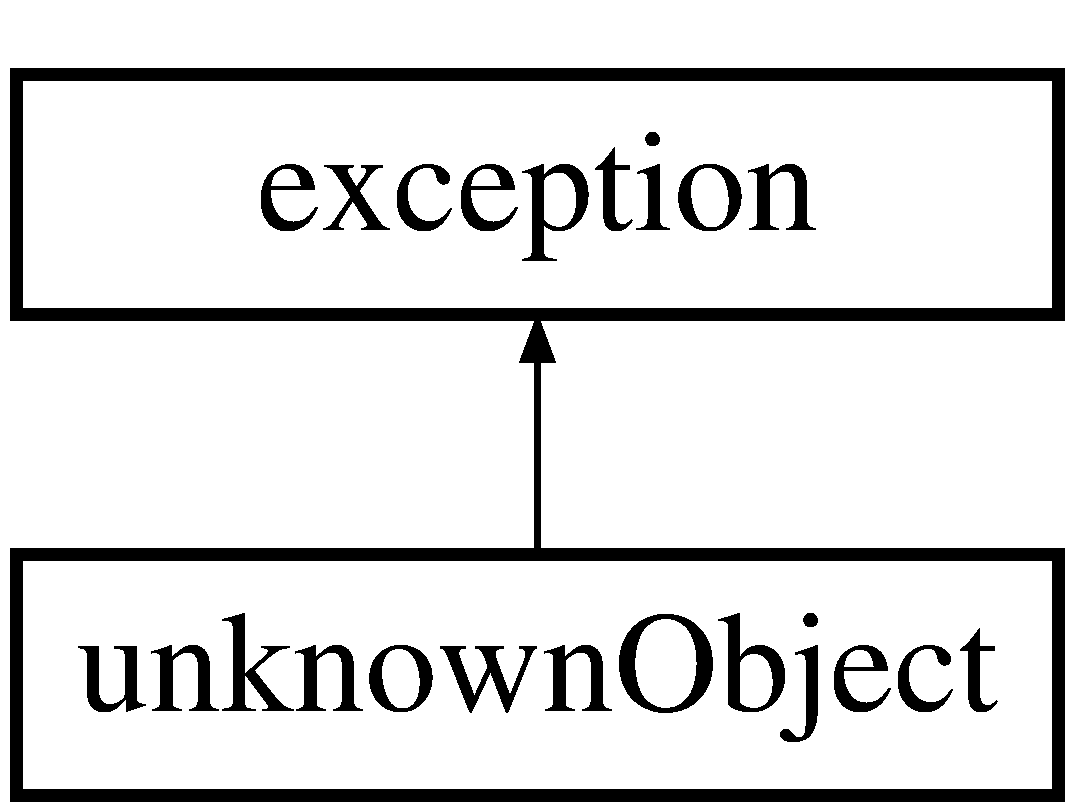
\includegraphics[height=2.000000cm]{classunknown_object}
\end{center}
\end{figure}
\subsection*{Public Member Functions}
\begin{DoxyCompactItemize}
\item 
\hyperlink{classunknown_object_ad8c2e8e7288078d86d3431e676d4dde4}{unknown\-Object} (std\-::string string)
\begin{DoxyCompactList}\small\item\em The constructor of the \hyperlink{classunknown_object}{unknown\-Object} exception. \end{DoxyCompactList}\item 
\hypertarget{classunknown_object_aae6ba49d97b52b42a4185c7a47021747}{const char $\ast$ \hyperlink{classunknown_object_aae6ba49d97b52b42a4185c7a47021747}{what} () const override}\label{classunknown_object_aae6ba49d97b52b42a4185c7a47021747}

\begin{DoxyCompactList}\small\item\em The \hyperlink{classunknown_object_aae6ba49d97b52b42a4185c7a47021747}{what()} method of an exception returns a string stating the exception. \end{DoxyCompactList}\end{DoxyCompactItemize}


\subsection{Constructor \& Destructor Documentation}
\hypertarget{classunknown_object_ad8c2e8e7288078d86d3431e676d4dde4}{\index{unknown\-Object@{unknown\-Object}!unknown\-Object@{unknown\-Object}}
\index{unknown\-Object@{unknown\-Object}!unknownObject@{unknown\-Object}}
\subsubsection[{unknown\-Object}]{\setlength{\rightskip}{0pt plus 5cm}unknown\-Object\-::unknown\-Object (
\begin{DoxyParamCaption}
\item[{std\-::string}]{string}
\end{DoxyParamCaption}
)}}\label{classunknown_object_ad8c2e8e7288078d86d3431e676d4dde4}


The constructor of the \hyperlink{classunknown_object}{unknown\-Object} exception. 

Creates a string which specifies what object is unkown 

The documentation for this class was generated from the following files\-:\begin{DoxyCompactItemize}
\item 
Exception.\-h\item 
Exception.\-cpp\end{DoxyCompactItemize}

%--- End generated contents ---

% Index
\newpage
\phantomsection
\addcontentsline{toc}{part}{Index}
\printindex

\end{document}
